\chapter{Related Work}

%% TODO make better introduction for the chapter. 

\section{Background} \label{background}
This section describes the background of this proposal and contains information that is available but might not be known by students and readers. 

\subsection{Introduction into GUI Testing}
Ever since the first line of software is written, testers are testing its workings. While in the early day of software, the \acrfull{ui} was mainly terminals based or a set of blinking LEDs \cite{altair8800} \footnote{For example the ALTAIR 8800 computer \cite{altair8800}}, today we have an ever-increasing amount of \acrfull{gui} applications. Testings a GUI application is labour intensive and costs a lot of money \cite{gui-history}.

Initially, testers were using \acrfull{cr} software to automate their work. A tester would record a test scenario into the CR software, and then the CR software will execute the test case when needed. Using CR software, the time required to retest software decreases; however, the big downside is that when software changes, so must the recorded scripts \cite{gui-history}.

Then came \acrfull{mbgt}. With MBGT, the GUI elements and behaviour are abstracted on a higher level. The created models are used to generate abstract test cases. Those abstract test cases need to be mapped or transformed to get concrete test cases that are executed on the SUT. The downside of MBGT is the effort required to create the models and the need to have formal modelling expertise. Formal modelling expertise is not needed with the latest evolution in test automation: model inference. 

The \emph{model inference}, also known as model extraction and GUI Ripping \cite{gui-ripping}, is the current state-of-the-art approach to automate GUI testing \cite{gui-history}. Inferred models are state graphs based on the GUI of the SUT. There are two ways to generate inferred models; the first is a static approach where the source code of the  SUT is used to create a GUI model. The second is a dynamic approach where the GUI state is captured and extracted while being executed. 

The static approach has several downsides. First, the source code must be available, which is not always the case and secondly, it is challenging to capture behaviour based on the GUI source code. For example, with HTML, it is easy to generate a model; however, its behaviour is either in Javascript or server code.  It is possible to overcome those stumbling blocks by executing the SUT.
    
As for the Dynamic approach, it captures the model during test execution. The automated test tool interacts with the SUT in a scriptless and random way. This random scriptless approach is called \emph{Monkey testing}. Usually, test monkeys have no idea in which state the SUT is in and what type of input is allowed. It is therefore essential to make the test monkey smarter. A "smart test monkey" can be achieved by making them "see" the UI elements (Section \ref{data-retrieval}). Section \ref{testar-testauto} will give more details about how TESTAR is using smart test monkeys.

\subsection{What is TESTAR?} \label{what-is-testar}
TESTAR - or TEST* - is an automated software testing tool for the GUI level \cite{testar-about}. TESTAR started within the context of the \acrfull{fittest} project. TESTAR is open-source, the source code is published on GitHub \footnote{ \url{https://github.com/TESTARtool/TESTAR\_dev}}. A screenshot of the TESTAR tool is displayed in Figure \ref{fig:testar}.

\bigskip
\begingroup
\captionsetup{type=figure}
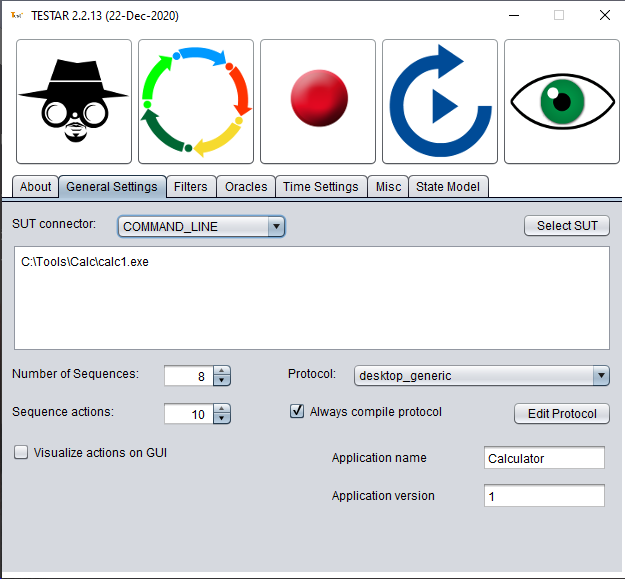
\includegraphics[scale=0.5]{images/testar.png}
\captionof{figure}{Screenshot of the TESTAR tool}\label{fig:testar}
\endgroup

TESTAR has several \emph{execution modes} in which it interacts with the SUT \cite{testar-manual}. From left to right, in figure \ref{fig:testar}, those are Spy, Generate, Record, Replay and View mode.

The \emph{Spy} mode allows the user to inspect a SUT and analyse how TESTAR is interpreting the widgets on the screen. Figure \ref{fig:calc-spy} shows the Windows calculator in spy mode. Dots on the GUI indicate actions that TESTAR could execute to interact with the SUT. Furthermore, within TESTAR, it is possible to filter out actions. Then, TESTAR will not execute those actions. The filtered actions are marked with a grey-coloured dot. A list with properties about the widget is shown when hovering, as well as a unique identifier of the current \emph{state}, more information about the state and the unique identifier can be found at section \ref{gui-state}.\par

\bigskip
\begingroup
\captionsetup{type=figure}
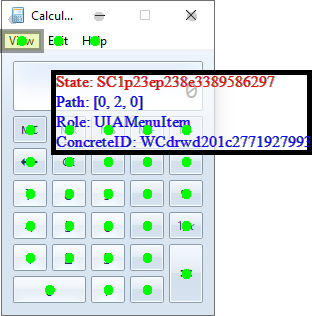
\includegraphics{images/calc-state.png}
\captionof{figure}{Screenshot of the Calculator with TESTAR Spy}\label{fig:calc-spy}
\endgroup

In the \emph{Generate} mode, TESTAR will start testing the specified system. Section \ref{testar-testauto} gives more details about TESTAR test automation.

The \emph{Record} mode allows a tester to record a test sequence manually. In the \emph{Replay} mode, existing test execution can be re-executed and lastly, the \emph{View} mode allows existing test executions to be viewed.

\newpage
\subsubsection{TEST automation} \label{testar-testauto}
TESTAR works without test scripts. Instead, it uses GUI Ripping and Monkey testing techniques. \emph{GUI Ripping}, first introduced by Memon et al. \cite{gui-ripping}, is a process to obtain the GUI's structure and execution behaviour automatically. As for \emph{Monkey testing}, it is a process in which decisions (interactions with the GUI) are randomly made. Section \ref{data-retrieval} will give more insights into GUI Ripping.

TESTAR is using a flow to execute tests on the SUT. This flow is as follows:
\begin{samepage}
\begin{enumerate}
    \item Start the SUT
    \item Scan the GUI and obtain the state (Section \ref{gui-state})
    \item Finding and selecting an action to execute
    \item Evaluate state with a test oracle (Section \ref{test-oracles})
    \item Stop the SUT when no actions are left to be executed or restart the SUT when more sequences are required.
\end{enumerate}
\end{samepage}

\bigskip
\begingroup
\captionsetup{type=figure}
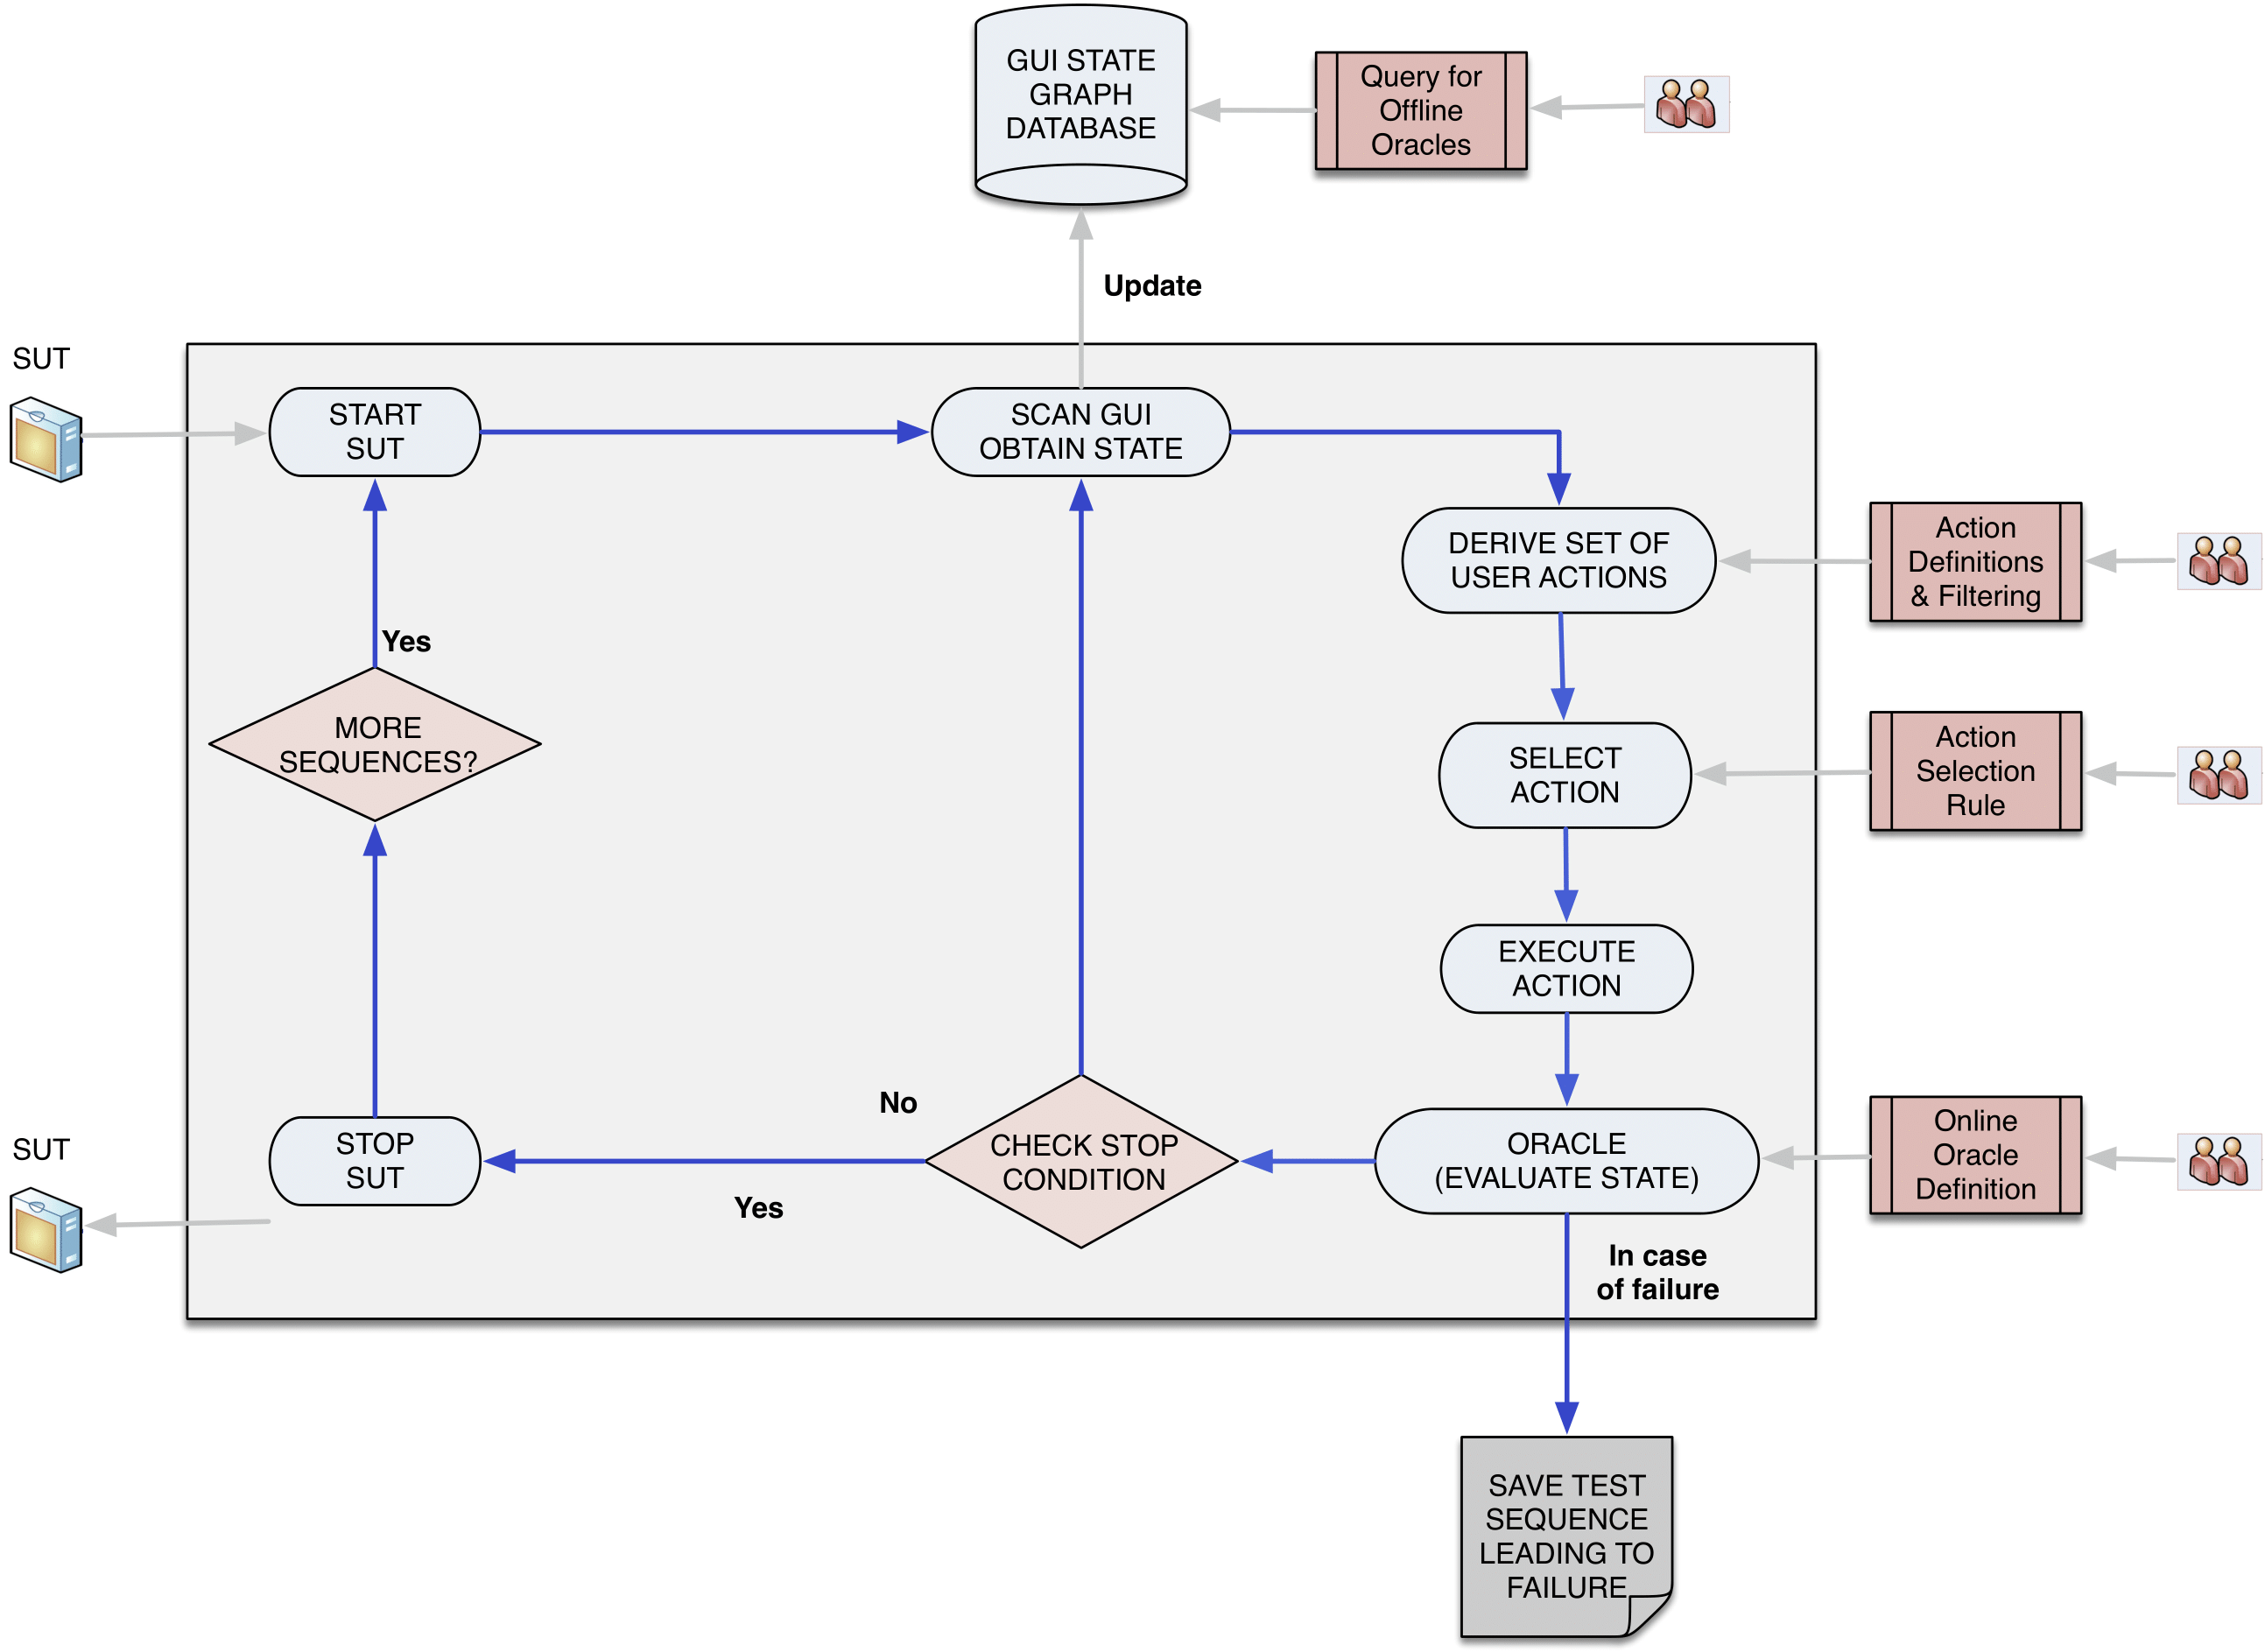
\includegraphics[scale=0.36]{images/testar-test-cycle.png}
\captionof{figure}{TESTAR test cycle \cite{testar-presentation}}\label{fig:testar-test-cycle}
\endgroup

Figure \ref{fig:testar-test-cycle} shows the flow graphically \cite{VosAho2021}. The test specialist needs to provide SUT details to TESTAR, like which actions should not be executed, and devise a mechanism that defines which SUT behaviour is correct and which is not, named a test oracle (Section \ref{test-oracles}). 

\subsection{How is the SUT tested} \label{test-oracles}
When software is tested, a method is needed to check the correct behaviour of the SUT. The method of checking is formally known as a \emph{test oracle} \cite{testOracles}. 

Outside the TESTAR context, an example of a test oracle could be a \emph{assertion} in software code. An assertion is a boolean expression created in a program by a software developer which checks the program's behaviour during run-time \cite{barr2014oracle}. Assertions can also be used in unit tests as displayed below on Listing \ref{code:assert}. 

%% do not indent code since it indents its extra in the LaTeX output
\begin{lstlisting}[language=Java, caption=Example assertion, label=code:assert]
@Test
public void testAdd(){
    Calculator sut = new Calculator();

    int expected = 3;
    int actual = sut.Add(1,2);

    Assert.assertEquals(expected, actual);
}
\end{lstlisting}

TESTAR comes with some test oracles out-of-the-box. Without any configuration, TESTAR will recognize crashes and unresponsiveness. It is also able to validate the GUI state with suspicious text. For example, a test sequence will fail when the title of a widget contains the word 'exception'. The input for the suspicious text is a regular expression that can be adjusted by the TESTAR user \cite{VosAho2021}. 

\subsubsection{Online and Offline Test oracles}
Test oracles come in two variants, \emph{online} or \emph{on-the-fly} test oracles and \emph{offline} test oracles \cite{VosAho2021}. With online test oracles, the state under test is being asserted for any anomalies during test execution. For example,  an online test oracle inspects the URL to check for any information being exposed in the query string. Offline test oracles will look into stored data - like logs - to find anomalies after test execution. For example, offline test oracles can inspect all the visited URLs to check for any exposed information in the query strings.

The two test oracle variants are complementary to each other and can run side by side. However, each variant comes with its strengths and weaknesses. The online test oracle takes up computation time because it inspects the state during test execution. This inspection of state slows down the test execution and may become an issue with time-critical SUTs. On the other hand, some issues - like the SUT becoming unresponsive - can only be checked during test execution. An offline test oracle is inspecting the gathered data after test execution has finished. Especially with larger data sets, this can become helpful. Inspecting the data may run in parallel, which can speed up the test oracle. Additionally, when developers create new offline test oracles, they can inspect the recorded data instead of executing a new test run \cite{de2019offline}.

\subsection{How is data retrieved} \label{data-retrieval}

Section \ref{testar-testauto} discussed how TESTAR is using GUI ripping to obtain the GUI's structure. A GUI consists of a non-empty set of UI components, known as \emph{widgets}. Examples of widgets are Windows or buttons; more examples can be found in Table \ref{tables:widgets} \cite{VosAho2021}. 

\begingroup
\captionsetup{type=table}
\begin{tabularx}{\textwidth}{ 
  | >{\raggedright\arraybackslash}X 
  | >{\raggedright\arraybackslash}X 
  | >{\raggedright\arraybackslash}X | }
    \hline
    Windows & Menus & Controls \\
    \hline
    \hline
    main windows & menu bars & buttons \\
    child windows & dropdown menus & textboxes \\
    popup windows & context-aware menus & links \\
    && radio buttons \\
    && checkboxes\\
    && dropdown select boxes\\
    && sliders\\
    && tabs\\
    && scrollbars \\
    \hline
\end{tabularx}
\captionof{table}{Example of GUI widgets \cite{VosAho2021}}\label{tables:widgets}
\endgroup

The widgets are structured hierarchically in a \emph{widget tree}. Each node in the tree is a widget with its related properties, such as the title, position and role. In figure \ref{fig:widget-tree} a compact widget tree is shown for the calculator. 

\bigskip
\begingroup
\captionsetup{type=figure}
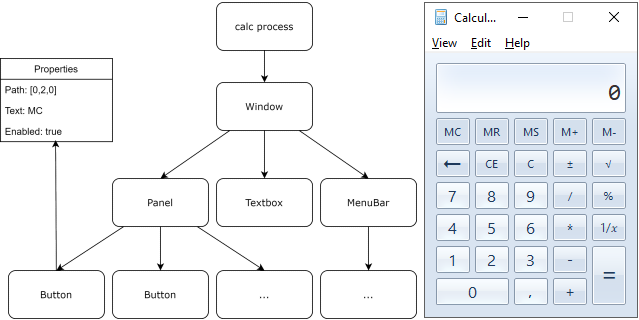
\includegraphics[scale=0.7]{images/calc-tree.png}
\captionof{figure}{A compact version of a widget tree for the calculator.}\label{fig:widget-tree}
\endgroup

\subsection{Widget data API}

In order to retrieve data from a SUT, TESTAR is making use of external APIs to access widgets that are part of the GUI \cite{thesisMulders}. TESTAR is using three different APIs.

In order to test a desktop application, TESTAR makes use of the Windows Automation API. The purpose of the Windows Automation API is to expose rich information about UI elements\cite{win-api-info}. For web applications, TESTAR uses Selenium Chromedriver. The Chromedriver is a tool for automated testing. It provides capabilities for navigating through web pages, user input, and JavaScript execution \cite{chrome-driver-info}. The latest API that TESTAR is using is Appium. Appium is a test automation tool for native, mobile web, and hybrid applications on iOS mobile, Android mobile, and Windows platforms \cite{appium-info}.

\subsection{GUI State} \label{gui-state}
In the previous sections, the widget tree is discussed and how the widgets are retrieved. In the widget tree, all the GUI elements with their properties are captured. The widget tree represents the state of the GUI when it has stopped executing any action. The GUI is at 'rest'. When an action is executed, the GUI can change, going to a new state. In figure \ref{fig:state-actions} the state change is represented in a small graph. 
\bigskip
\begingroup
\captionsetup{type=figure}
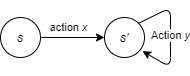
\includegraphics{images/state-action.png}
\captionof{figure}{An graph with two states and two actions.}\label{fig:state-actions}
\endgroup

The graph is a directed graph since every action changes the GUI from one state to the other. An action may lead to the same state, see figure \ref{fig:state-actions} action \textit{y}. However, that would mean that the action does not do anything or TESTAR does not indicate a change. For example, the GUI changes but not the property corresponding to the change is not included in the widget tree.

The universe of states and actions of the SUT's GUI makes up an inferred model. More information about the inferred model and how they are created can be found in section \ref{inferred-model}.

\subsection{How is data persisted}

TESTAR is using a database to store and retrieve state model data. Gier and Kager investigated which data storing solution would be beneficial to TESTAR \cite{GierKager}. The data solution must comply with six requirements. Generally speaking, the requirements were as follows: an open-source graph database with a straightforward query mechanism. The conclusion was that OrientDB was the best solution that met all the requirements.

\begin{samepage}
OrientDB is a Multi-Model NoSQL \acrfull{dbms} that combines four models \cite{orientDbModeling}:

\begin{itemize}
    \item \hyperlink{db:key-value}{Key/Value}
    \item \hyperlink{db:document}{Document}
    \item \hyperlink{db:graph}{Graph}
    \item \hyperlink{db:object}{Object}
\end{itemize}
\end{samepage}

A \hypertarget{db:key-value}{\emph{Key/Value}} is the simplest model and allows storing information (value) that is accessible with a key. Key/Values can be grouped into \textit{buckets}. However, OrientDB supports richer models in the form of document and graph elements.

A \hypertarget{db:document}{\emph{document}} is a schema-less set of key/value pairs. The \emph{key} allows access to the corresponding value. OrientDB allows the developer to store documents into \emph{clusters}. Relations between document are either embedded into other document or \emph{linked} to each other. Someone familiar with relational databases can view a cluster as tables, a document as the row and the key/value pairs are columns.

The \hypertarget{db:graph}{\emph{graph}} is a model consisting of \emph{Vertices} and \emph{Edges}. Vertices are the nodes in the graph, and the edge is the link between those nodes. In TESTAR terminology, a vertex represents state, and the edge is an 'action' from one state to the next. A Vertex consists of three elements: a unique identifier, a set with incoming Edges and outgoing Edges. An edge consists of four elements: a unique identifier, an incoming vertex (\emph{head}), an outgoing vertex (\emph{tail}) and a label that describes the relationship between the head and tail vertex.\par

The last model is the \hypertarget{db:object}{\emph{object}} that supports inheritance, like in the Object-Oriented programming paradigm.\par

Despite being a NoSQL database, OrientDB does support SQL as a query language \cite{sql-lang} albeit that it does not support all SQL statements. The majority of developers have experience with SQL \cite{sql-stats}, and as a result, new developers and students can start querying the TESTAR data and start expanding its features.\par

In addition to TESTAR, other applications can query the state model data in the OrientDB database as well. For example, developers and students can create external tools for a single purpose, like a state model difference application. When building external tools, the TESTAR application can be kept small and focus upon one objective: testing GUI applications. 

\section{Related work} \label{releatedWork}
This section covers an overview of the material that is the direct foundation for this research proposal.

\subsection{Inferred model} \label{inferred-model}
The master thesis by Mulders had two significant outcomes. The first is an inferred model module, and the second is the visualisation of the inferred models \cite{thesisMulders}. The visualisation model is a web-based application that shows the inferred model with screenshots and properties. Although the visualisation module becomes required when we want to visualise the result of the change-detection software, it is not necessary to go into depth in this document. This section will discuss what an inferred model is and how they are generated. 

The GUI state was discussed in section \ref{gui-state}. The section ended with the sentence that the universe of states and actions of the SUT's GUI makes up the inferred model. The inferred model is a directed graph showing the GUI-state of the application and the transactions between states. The vertex of the graph represents the GUI-state. Each vertex has a set of incoming and outgoing edges, called the actions. 

Figure \ref{fig:state-model} shows the result of the inferred model in the visualisation module.

\bigskip
\begingroup
\captionsetup{type=figure}
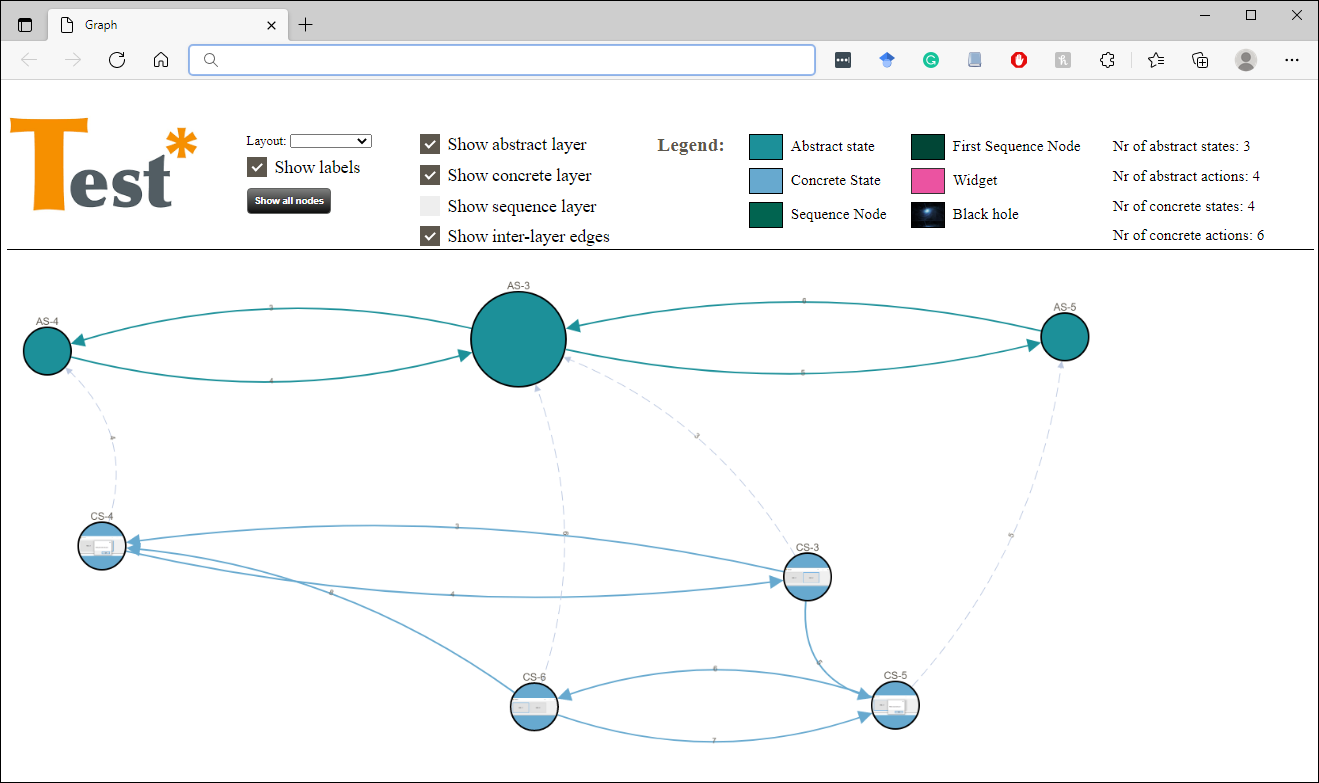
\includegraphics[scale=0.38]{images/state-model.png}
\captionof{figure}{an inferred model in the visualisation application}\label{fig:state-model}
\endgroup

In figure \ref{fig:state-model} two models can be observed. The first model, indicated by the AS text, shows the abstract model. The second, indicated by the CS text, shows the concrete GUI states. 

\subsubsection{Concrete model}
The concrete model contains all the data that could be retrieved from the GUI. The identification key uses a hash calculated over all the properties. Aside from the widget's properties, the concrete models also contain a screenshot of the GUI for each state \cite{thesisMulders}.

Figure \ref{fig:concrete-node} shows an example of a node in the concrete model. Upon selecting a node, the properties of the node show, including the screenshot taken during the test. The grey dotted line, indicated with the letter 'a', shows the connection with the abstract node, see section \ref{abstract-model} and figure \ref{fig:abstract-model} for more details. The two outgoing edges, indicated with the letter 'b', shows the two actions available in this state. The incoming edge, indicated with the letter 'c', shows how the state was reached. 

\bigskip
\begingroup
\captionsetup{type=figure}
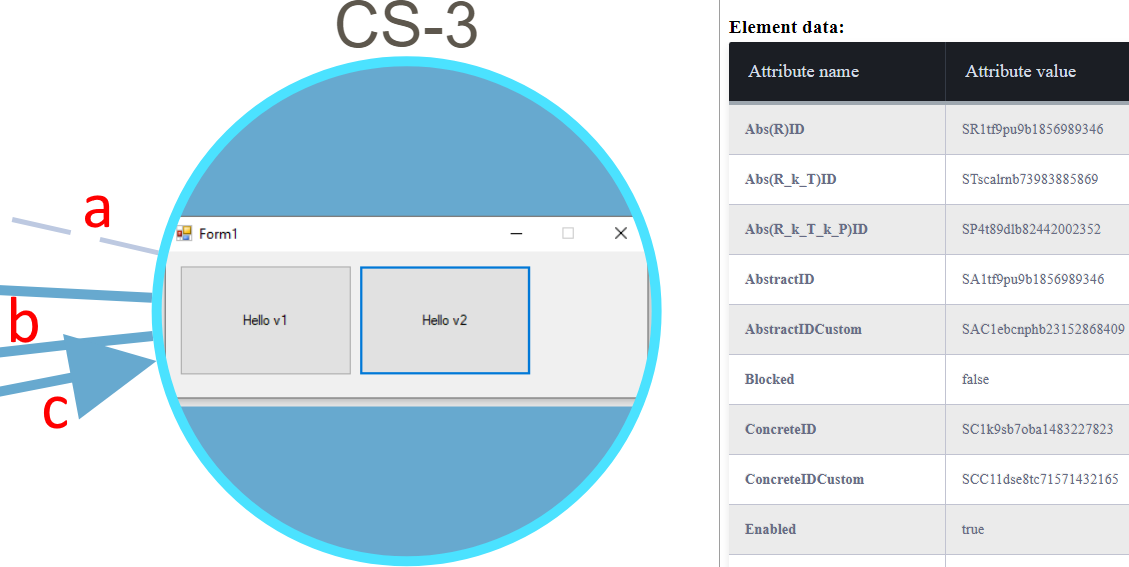
\includegraphics[scale=0.5]{images/concrete-model.png}
\captionof{figure}{A node from the concrete model}\label{fig:concrete-node}
\endgroup

\newpage
\subsubsection{Abstract model} \label{abstract-model}
Since the concrete models containing all the data from a GUI-state, they can become quite large.  Therefore an abstraction model is made \cite{thesisMulders}. Figure \ref{fig:abstract-model} shows an example of such a abstract node. The grey lines (from CS-3, CS-6 to AS-3) indicates which concrete state is abstracted. The properties of the abstract node are displayed, what the identifier is and which concrete state(s) it represents.

\bigskip
\begingroup
\captionsetup{type=figure}
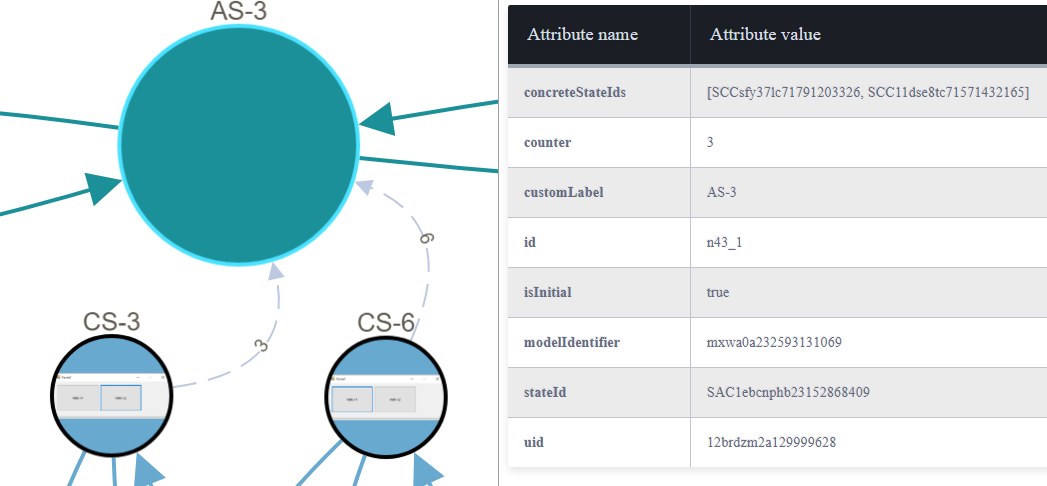
\includegraphics[scale=0.5]{images/abstract-model.png}
\captionof{figure}{A node from the abstract model}\label{fig:abstract-model}
\endgroup

\subsubsection{State identifiers} \label{state-identifiers}
Every state must have a unique id for identification. The identifier is calculated with the data from the widget tree. 

TESTAR uses a hashing algorithm that works as follows: the widgets' properties are concatenated and hashed. The outcome will be used as the identifier for a widget. The hashes from the widget in the widget tree are then combined and hashed to create an identifier for the GUI state \cite{VosAho2021}. The TESTAR's algorithm is similar to how a Merkle tree works, more information can be found at section \ref{merkle-tree}.

To identify the state (and actions), TESTAR calculates two state identifiers; an abstract and concrete state identifier. For the concrete state identifier, all the properties of a widget are used. For the abstract identifier, a subset of the properties is used. It is configurable which properties are used for the abstract identifier. By default the properties \textit{role}, \textit{title}, \textit{position} and \textit{enabled} are utilised \cite{VosAho2021, thesisMulders}.

When running TESTAR, it is possible to configure which widget properties should be used for the abstract state identifier. Figure \ref{fig:advance} shows the selection dialogue in which the user can select the properties for the abstract identifier.

\subsection{Merkle tree} \label{merkle-tree}
A Merkle tree is a hash tree data structure where a hash can identify each vertex. \cite{merkle-tree} The cryptographic hash is calculated by taking the hashes of the descendant vertices, combining them, and calculating a new hash from the combination. 

As written in the previous section (\ref{state-identifiers}), TESTAR's way of calculating the identification id for a widget or a GUI state is similar to that of the Merkle tree vertex. The hashed id for a widget is based on the hashed property values. Figure \ref{fig:merkle-tree} shows an example of a Merkle tree about how the GUI state identification id is calculated. The corresponding widget tree (Figure \ref{fig:widget-tree}), where the Merkle tree is based, is shown in the top right corner.

Although a Merkle tree usually is a binary tree \cite{merkle-tree}, having more than two descendant vertices is not considered a problem since the same Merkle-tree principle can be applied.

\bigskip
\begingroup
\captionsetup{type=figure}
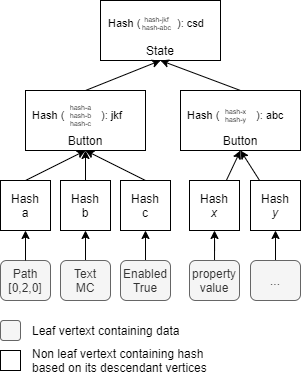
\includegraphics[scale=0.8]{images/merkle-tree-example.png}
\captionof{figure}{An short Merkle tree example based on a widget tree}\label{fig:merkle-tree}
\endgroup

\subsubsection{How is an inferred model created?}
This research focuses itself on the outcome of the obtain step as illustrated in figure \ref{fig:obtain-state-graph}, which is the top right part of figure \ref{fig:testar-test-cycle}.

\bigskip
\begingroup
\captionsetup{type=figure}
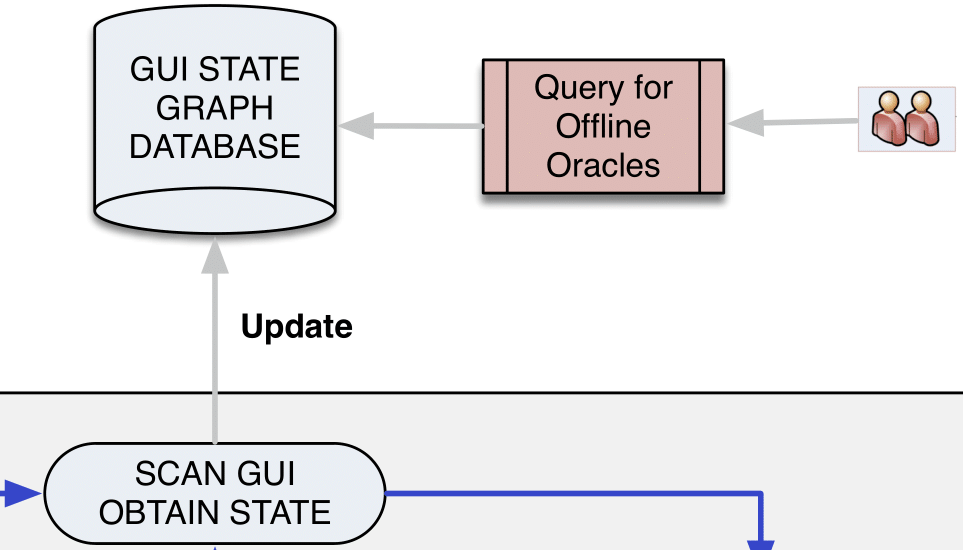
\includegraphics[scale=0.4]{images/obtain-state-graph.png}
\captionof{figure}{The focus of this research proposal \cite{testar-presentation}}\label{fig:obtain-state-graph}
\endgroup

Generating the inferred model starts when TESTAR start testing the SUT. After an action has been executed successfully, the state of the GUI is sent to the inferred model module. When the state is reached without action, it is marked as the initial state. 

The inferred model module generates the abstract and concrete state's and saves those in the model. The model is persisted in the OrientDb database. At last, a deterministic model check is being performed and saved \cite{testar-code}.

\subsection{State model difference}
The \verb|StateModel.Difference| package, added by Pastor Ricós\cite{stateDiff}, offers a proof of concept for calculating differences between the inferred state models. For the comparison, the \verb|abstractStateId| is used. 

Pastor Ricós difference algorithm\cite{stateDiff} outputs two classification of changes between two models: added and removed state. Let $A$ be a set of \verb|abstractStateId|s of version 1 of the SUT, and let $B$ be a set of \verb|abstractStateId|s of version 2 of the SUT. The removed states can be written as
\[A-B = \lbrace x | x \in A \wedge x \notin B \rbrace\]
the states that are added can be written as
\[B-A = \lbrace x | x \in B \wedge x \notin A \rbrace\]

\begingroup
\captionsetup{type=figure}
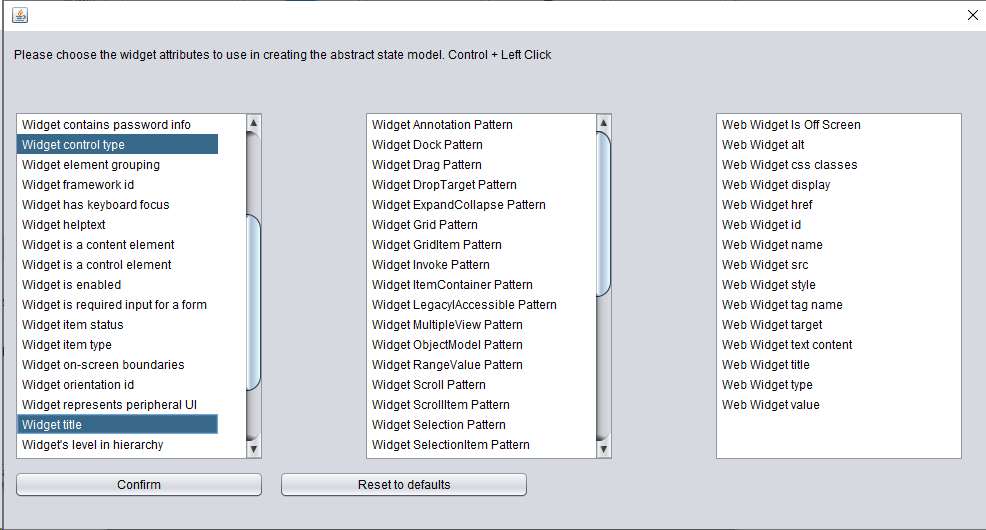
\includegraphics[scale=0.5]{images/attributes-state-model.png}
\captionof{figure}{Select widgets attributes for the abstractStateId}\label{fig:advance}
\endgroup

Using the \verb|abstractStateId| is excellent for the proof of concept and preliminary change detection, 
However, its boolean nature in which state exists or not can result in many 'false' changes. For example, when a widget is moved, the change detection should result in an altered state, not a removed and added state. 

Section \ref{state-identifiers} discussed how identifiers are generated, since the differences are calculated based on the \verb|abstractStateId| selecting the correct widget attributes is vital. Choosing too few attributes could result in conflicting differences like the same actions are removed and added. Choosing too many attributes could trigger a change in even the tiniest detail. Choosing the widget attributes can be done with the 'Advance' screen under the State model tab. See Figure \ref{fig:advance}.

For the research proposal, an experiment application is created; the two-buttons app. With the two-buttons app, it was possible to experiment with various TESTAR settings. The application is shown in figures \ref{fig:exp-v1}, \ref{fig:exp-v2} and \ref{fig:exp-v3}. As one can observe, the differences between version 1 and version 2 are the added button with the label 'Hello v2' and between version 2 and 3 the buttons' colour and position. 

\begin{tabularx}{\textwidth}{@{} 
   >{\raggedright\arraybackslash}X
   >{\raggedright\arraybackslash}X  }
    \begingroup
    \captionsetup{type=figure}
    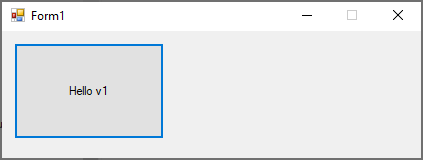
\includegraphics[scale=0.60]{images/exp-v1.png}
    \captionof{figure}{Version 1 of the experiment application}\label{fig:exp-v1}
    \endgroup
    &
    \begingroup
    \captionsetup{type=figure}
    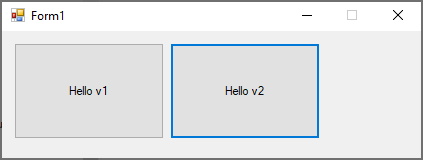
\includegraphics[scale=0.60]{images/exp-v2.png}
    \captionof{figure}{Version 2 of the experiment application}\label{fig:exp-v2}
    \endgroup
    
    \\
    
    \begingroup
    \captionsetup{type=figure}
    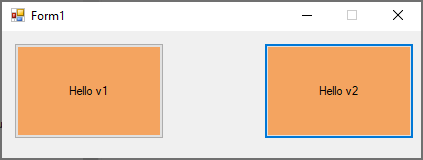
\includegraphics[scale=0.6]{images/exp-v3.png}
    \captionof{figure}{Version 3 of the experiment application}\label{fig:exp-v3}
    \endgroup
\end{tabularx}


However, a different result is displayed when using 'widget title' and 'widget control type' as widget attributes for the abstract states. Namely, the button with the label 'Hello v1' is removed between the first two versions. The buttons labelled 'Hello v1' and 'Hello v2' are added. Between versions 2 and 3, no differences are observed.

This change difference outcome can be explained by the way the proof of concept is working. The widget tree of version 1 contains one button, whereas the widget tree of version 2 contains two buttons. Therefore both the abstract and the concrete identifiers are different for both widget trees. The proof of concept change detection checks whether the abstract identifier of version 1 can be found in version 2, which it cannot, so the state is marked as removed. The state of version 2 can likewise not be found in version 1 so that state is marked as new.

The chosen widget attributes explain the absence of changes between versions 2 and 3. Neither the title nor the control type has changed. Since those attributes were used for the abstract identifier, TESTAR did not detect a change. 

In section (\ref{research-questions}), the research questions are discussed. Of course, one of the questions will investigate how the change detection algorithm must be implemented. The findings of the two-button app should be considered, and the experiment should be adapted to contain different changes to test on. 

%\newpage
\subsection{TESTAR in containers}
A recent master thesis by Slomp explains how TESTAR can be integrated into a \acrfull{ci} environment \cite{thesisSlomp}. Slomp introduced TESTAR into the world of Docker and container and integrated TESTAR into an Azure DevOps pipeline. A pipeline is a collection of steps that can automatically build, test and release software. A container bundles all the software, configuration files and libraries together so that an application can run \cite{ms-container}. 

When TESTAR is being run within the Azure DevOps pipeline, the TESTAR GUI is not shown. Running TESTAR is not a problem. However, to analyse the outcome of TESTAR, the users need to install TESTAR and have access to the OrientDb database location. 

By moving the code for change detection and visualisation into a stand-alone web application, the user can analyse the outcome on their browser. Since TESTAR is wrapped into a container, the stand-alone tool will also be wrapped to provide the same infrastructure. Nevertheless, it is up to the IT administrator how they deploy the TESTAR suite. 

Additionally, to the user's benefit, a TESTAR developer can also benefit from the application's separation. Changes to either the separate application or TESTAR can be made without being conflicting with the other. Each tool can focus on one goal, while TESTAR can focus on testing GUI applications. 